\documentclass[]{scrartcl}
\usepackage[utf8]{inputenc}
\usepackage{graphicx}
\usepackage{amsmath}
\usepackage{float}

\title{Modellierung dynamischer Systeme  \\ Entwurf zur Bearbeitung der Praktikumsaufgabe 2}

\author{Maria Lüdemann und Birger Kamp}

\begin{document}

\maketitle

\begin{abstract}

\end{abstract}

\section{Allgemein}
Diese Praktikumsaufgabe beschäftigt sich mit dem Anwenden von DGLn bei der Modellierung von physikalischen Vorgängen. In dieser Aufgabe werden Satelliten Flüge zwischen der Erde und dem Mond , sowie diverse Pendelbewegungen modelliert.

\section{Teilaufgabe 1}
In dieser Aufgabe wird ein Satellit von der Erde losgeschickt. Zu modellieren ist der antriebslose Flug des Satelliten, sobald er die Position $x_{0}$ erreicht hat. Von dort beginnt der Satellit seinen antriebslosen Flug mit der Startgeschwindigkeit $v_{0}$ und dem Flugwinkel $\Theta$. Der Flug ist vereinfacht im zweidimensionalen Raum zu modellieren.

Es wurde eine MatLab-Skript \textit{Erdbahn.m} bereitstellt. Mit dem im Anschluss die Flugbahn des Satelliten visualisiert werden kann.

Abbildung \ref{fig:1_BezeichnerDiagramm} illustriert das Modell sowie die jeweiligen Bezeichner.
\begin{figure}[H]
\centering
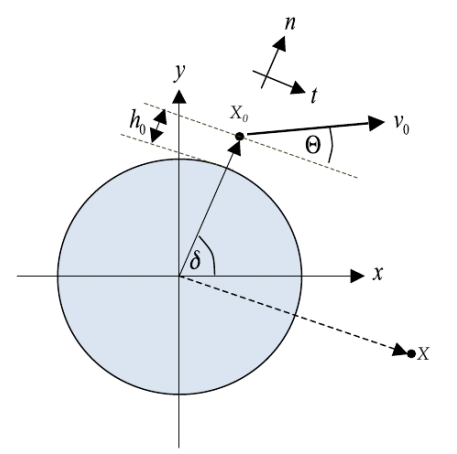
\includegraphics[width=0.5\linewidth]{./1_BezeichnerDiagramm}
\caption{}
\label{fig:1_BezeichnerDiagramm}
\end{figure}

\subsection{Gegebene Formeln und Konstanten}
Kraft auf den Satelliten
\begin{align}
\vec{F}_{S} = G * \dfrac{m_{E} * m_{S}}{r^2} * \vec{e}_{SE}
\end{align}

Erdradius
\begin{align}
r_{E} = 6378 km
\end{align}

Erdmasse
\begin{align}
m_{E} = 5,9736 * 10^{24} kg
\end{align}

Gravitationskonstante
\begin{align}
G = 66,743 * 10^{-12} m^{3} kg^{-1} s^{-2}
\end{align}

\subsection{Konfigurierbare Parameter}
Folgende Parameter müssen mindestens bei der Simulation konfigurierbar sein:
\begin{itemize}
\item $v_{0}$
\item $\Theta$
\item $\gamma$
\item $h_{0}$
\end{itemize}

\subsection{Erdachte Formeln}
Folgende Formeln wurden selbst erdacht, und sollen bei der Lösung behilflich sein:
\begin{align}
r = \sqrt{x^2 + y^2} \\
h = r - r_{E} \\
\vec{e}_{SE} = \dfrac{1}{\sqrt{x^2 + y^2}}* \begin{pmatrix}x\\y\end{pmatrix} = \dfrac{1}{r} * \begin{pmatrix}x\\y\end{pmatrix}
\end{align}

%TODO: Formeln ergänzen!
\subsection{Hinweise bei der Lösung mit MatLab}
\begin{itemize}
\item Die Simulation soll den Namen \textit{Erdorbits} haben.
\item In den Simulink-Schaltbildern sollen Vektorintegratoren verwendet werden. Das ist ein einfacher Integrator, der sein Eingangssignal aus einem Multiplexer erhält.
\item Die errechneten Bahnkoordinaten des Satelliten sollen von Simulink als getrennte x- und y-Werte in den MatLab-Workspace übergeben werden. Von dort werden sie visualisiert.
\item Sobald der Satellit die Erdoberfläche erreicht ($h=0$), soll die Simulink-Simulation beenden.
\item Es soll eine EM-Funktion \textit{Startposition} geben, die aus den Parametern $\gamma$, $h_{0}$ und dem Erdradius den Startpositionsvektor $x_{0}$ berechnet.
\item Es soll eine EM-Funktion \textit{vStart} geben, die aus $v_{0}$, $\Theta$ und $x_{0}$ soll der Startgeschwindigkeitsvektor berechnet werden. Der Vektor soll den Anfangswert als Weltkoordinaten enthalten. Dabei wird der Tipp gegeben, erst die Einheitsvektoren in Tangential- und Normalenrichtung ($\vec{n},\vec{t}$) aus $x_{0}$ zu konstruieren. Danach werden die Tangential- und Normalenkomponenten der Startgeschwindigkeit ($v_{t}$,$v_{n}$) berechnet. %TODO: Hier fehlt noch ein Satz, warte auf Mail
\item Es soll eine EM-Funktion \textit{Beschleunigung} geben, die aus der aktuellen Satellitenposition $\vec{x}$ die aktuelle Satellitenbeschleunigung berechnet.
\item Es soll eine EM-Funktion \textit{Kontakt} geben, die den Wert \textit{0} ausgibt, solange der Satellit sich über der Erdoberfläche befindet ($h > 0$), ansonsten gibt sie den Wert \textit{1} aus.
\item Die Simulink-Simulation soll ein Display haben, dass die bislang vergangene Zeit in Stunden anzeigt.
\end{itemize}

\subsection{Durchführung 1}
Im ersten Experiment sollen die Werte $\gamma = 30^\circ,\ h_{0} = 400km$ und $\Theta=0^\circ$ angenommen werden. Die Startgeschwindigkeit $v_{0}$ soll so bestimmt werden, dass der Satellit in einer Kreisbahn auf gleicher Höhe fliegt (Tipp: ca. $7,4 - 8,5 km*s^{-1}$). Außerdem soll bestimmt werden, wie lange eine Erdumkreisung dann dauert (Tipp: ca. $1 - 2h$).

\subsection{Durchführung 2}
Im zweiten Experiment beträgt die Simulationszeit $1 * 10^6s$ betragen. Es soll $v_{0}$ bestimmt werden, sodass der Satellit gerade der Erde entflieht (Tipp: ca. $10 - 11 km*s^{-1}$).

\subsection{Durchführung 3}
Im dritten Experiment sollen die Werte $\gamma = 30^\circ$ und $\Theta = 0^\circ$ angenommen werden. Es sollen $h_{0}$ und $v_{0}$ so bestimmt werden, dass die Kreisbahn des Satelliten genau 1 Tag dauert. (Tipp: $h_{0} \approx 40000 km$ und $v_{0} \approx 3 km *s ^{-1}$)

%TODO: Es fehlt ein Diagramm das zeigt, wie der Mond zur Erde besteht und wie der Winkel dort benannte wird.
\section{Teilaufgabe 2}
Zu dieser Teilaufgabe wird das Simulink-Modell aus Teilaufgabe 1 kopiert. Nun soll der Satellit nicht mehr um die Erde kreisen, sondern zusätzlich auch um den Mond.

Zur Visualisierung des Modells wurde ein MatLab-Skript \textit{ErdMondBahn.m} bereitgestellt.

\subsection{Zusätzliche Konstanten}
Mondposition(fest)
\begin{align}
x_{M} = (0,380000)^T km
\end{align}

Mondmasse
\begin{align}
m_{M} = 7,3480 * 10^{22} kg
\end{align}

\subsection{Änderungen am Modell}
Im kopierten Simulink-Modell muss die EM-Funktion \textit{Beschleunigung} angepasst werden. %TODO: Wie muss sie angepasst werden?
Die Simulationszeit wird nun nicht mehr in Stunden, sondern in Tagen angegeben.

\subsection{Durchführung}
Es sind die Werte $\gamma_{0} = 30^\circ$ und $h_{0} = 150km$ gegeben.

Es müssen die Werte $v_{0}$ und $\Theta$ bestimmt werden, sodass der Satellit in einer 8-förmigen Schleife von der Erde startend um den Mond fliegt und zur Erde zurück fliegt. Es ist zu ermitteln, wie lange die Mission dauert.


\end{document}
